\chapter{消化道影像解剖}

消化道自口腔开始,往下依次为食管、胃、十二指肠、空肠、回肠、结肠,至肛门结束,为一弯曲的管道结构,本章将具体介绍胃,小肠及结肠的影像学检查方法及正常解剖结构。

\section{检查方法}

(一)胃CT准备方法

检查前一日晚上进易消化无渣饮食(稀饭、藕粉等)。检查当日空腹。检查前肌肉注射东莨菪碱20mg(有禁忌证者除外),出现口干症状后口服饮用水1000~1200ml,而后进行CT扫描。

(二)小肠CT准备方法

检查前三日禁做胃肠道钡剂造影检查。检查前一日中午行无渣半流质饮食,每2小时口服葡萄糖注射液500ml,至晚8∶00口服50%硫酸镁50ml,8∶30口服20%甘露醇250ml,晚10∶00再次口服5%葡萄糖注射液500ml。检查当日空腹。扫描前30min内口服肠道充盈混合溶液1000ml及饮用水1000ml,混合溶液配比方案为5%葡萄糖注射液500ml+20%甘露醇注射液250ml+饮用水250ml,扫描前肌内注射东莨菪碱注射液20mg(有禁忌证者除外),进行CT扫描。

(三)结肠CT准备方法

检查前三日禁做胃肠道钡剂造影检查。检查前一日中午行无渣半流质饮食,每2小时口服葡萄糖注射液500ml,至晚8∶00口服50%硫酸镁50ml,8∶30口服20%甘露醇250ml,晚10∶00再次口服5%葡萄糖注射液500ml。检查当日空腹。扫描前10min肌内注射东莨菪碱注射液20mg(有禁忌证者除外),然后嘱病人俯卧于担架床上,暴露肛门,将肛管插入肛门内4~6cm,缓慢注入温生理盐水1500~2000ml,然后将病人送至CT扫描床上,进行扫描。

扫描技术参数:120kV,平扫250~280mA,增强350~400mA,层厚:10mm,重建层厚1.25mm,间隔0.8mm。

扫描范围:即从膈顶至耻骨联合下缘。

扫描方法:平扫一次完成全腹扫描,增强行双期扫描,注射造影剂采用高压注射器,造影剂量100~120ml,注药速度3.0~3.5ml/s,增强动脉期采用Smart
PrepRX监测,监测点取肠系膜上动脉水平腹主动脉,当时间密度曲线峰值达50Hu时启动扫描,增强门脉期与第一期间隔时间25s。

图像后处理:将重建图像传至工作站,主要采用多平面重建(MPR)方法获得冠状位、矢状位及斜位重建图像,用MPVR观察血管、肠系膜淋巴结及后腹膜淋巴结,对于肠管迂曲时可采用曲面重建(CPR),阳性造影剂可用容积重建(VR)。

(四)MRI扫描方法

扫描开始前5min肌注山莨菪碱针剂2ml,减少肠道蠕动。运用体线圈,扫描序列为T\textsubscript{1}
W/SE-EPI/横断位(TR=792,TE=25),T\textsubscript{2}
W/TSE/横断位(TR=1800,TE=99),T\textsubscript{1}
W/SPIR/横断位(TR=500,TE=15),T\textsubscript{2}
W/SPIR/横断位(TR=1800,TE=80),T\textsubscript{2}
W/冠状位(TR=1875,TE=100),T\textsubscript{2}
W/SPIR/冠状位(TR=1875,TE=100),MIP重建/3D水成像。FOV为380~435,层厚10mm,间隔10mm。扫描范围由肝脏膈面至耻骨联合。必要时可静脉注射Gd-DTPA进行增强检查。

\section{横断面}

本节我们将自上而下逐层介绍在扫描过程中出现的消化道结构。

\begin{figure}[!htbp]
 \centering
 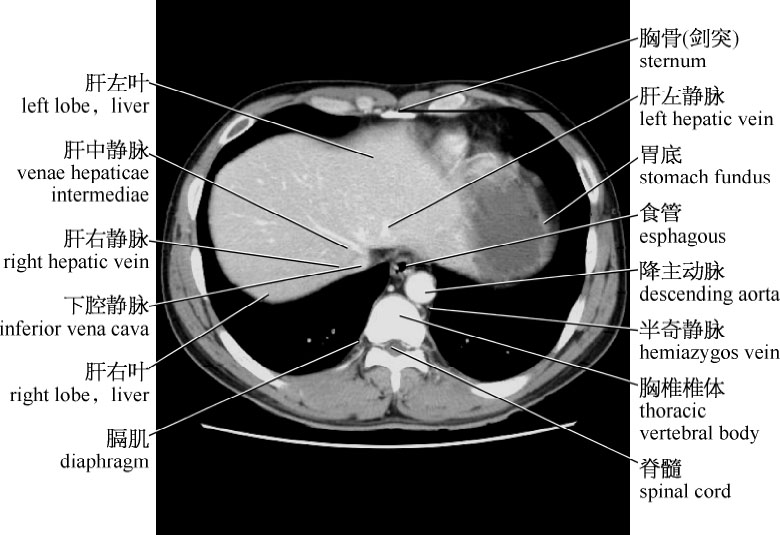
\includegraphics{./images/Image00166.jpg}
 \captionsetup{justification=centering}
 \caption{胃底}
  \end{figure} 
 \FloatBarrier

\begin{figure}[!htbp]
 \centering
 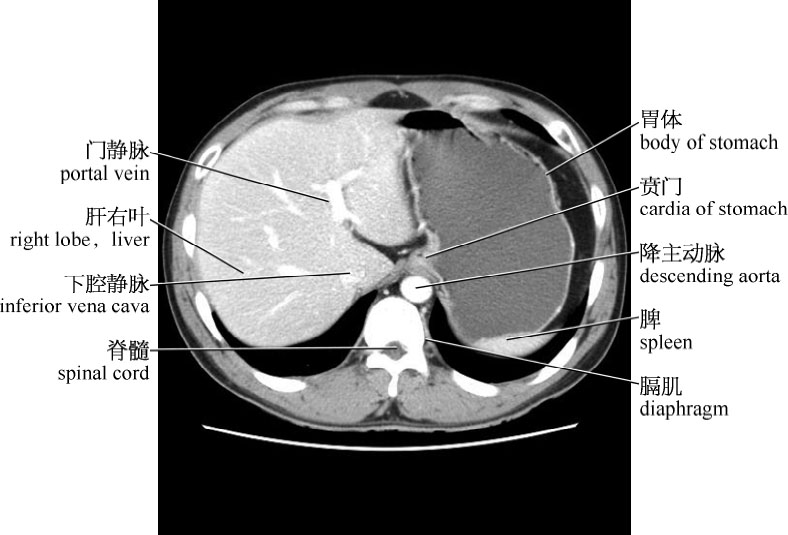
\includegraphics{./images/Image00167.jpg}
 \captionsetup{justification=centering}
 \caption{胃体上部与贲门}
  \end{figure} 
 \FloatBarrier

\begin{figure}[!htbp]
 \centering
 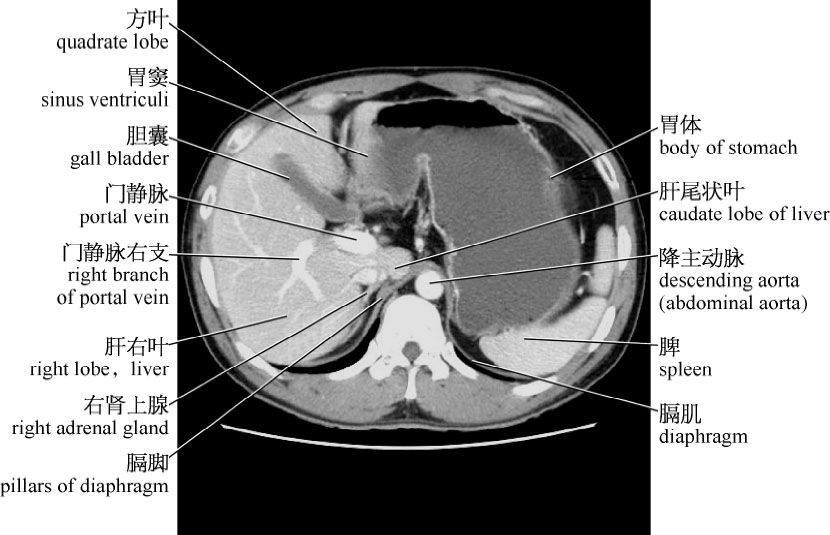
\includegraphics{./images/Image00168.jpg}
 \captionsetup{justification=centering}
 \caption{胃体与胃窦}
  \end{figure} 
 \FloatBarrier

\begin{figure}[!htbp]
 \centering
 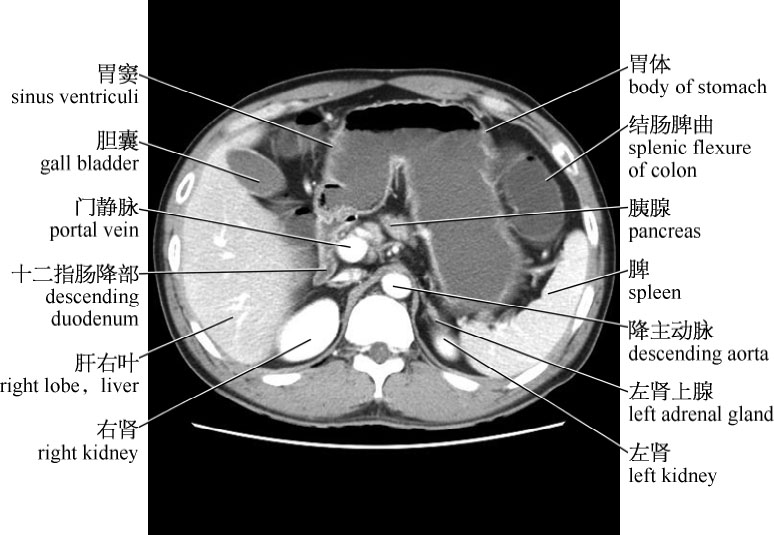
\includegraphics{./images/Image00169.jpg}
 \captionsetup{justification=centering}
 \caption{胃窦与十二指肠}
  \end{figure} 
 \FloatBarrier

\begin{figure}[!htbp]
 \centering
 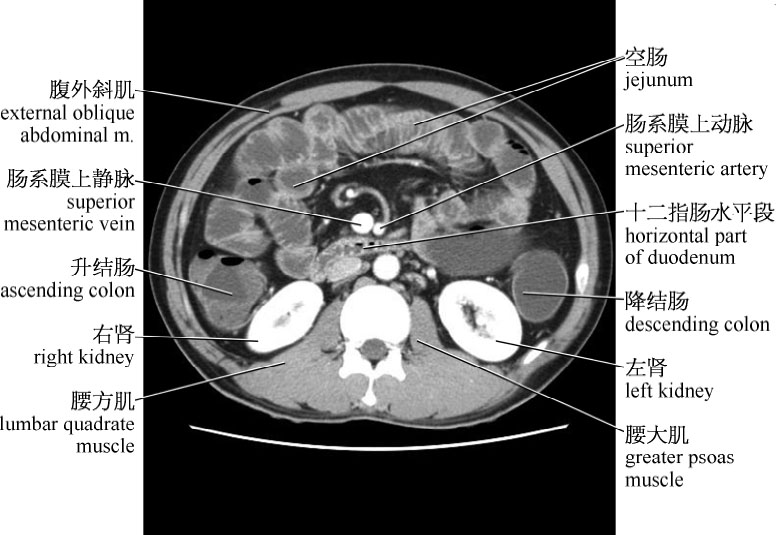
\includegraphics{./images/Image00170.jpg}
 \captionsetup{justification=centering}
 \caption{十二指肠与空肠}
  \end{figure} 
 \FloatBarrier

\begin{figure}[!htbp]
 \centering
 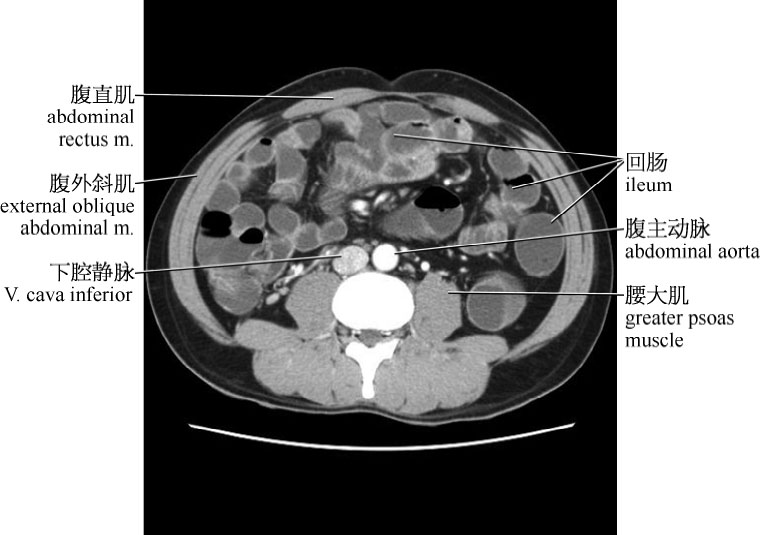
\includegraphics{./images/Image00171.jpg}
 \captionsetup{justification=centering}
 \caption{回肠}
  \end{figure} 
 \FloatBarrier

\begin{figure}[!htbp]
 \centering
 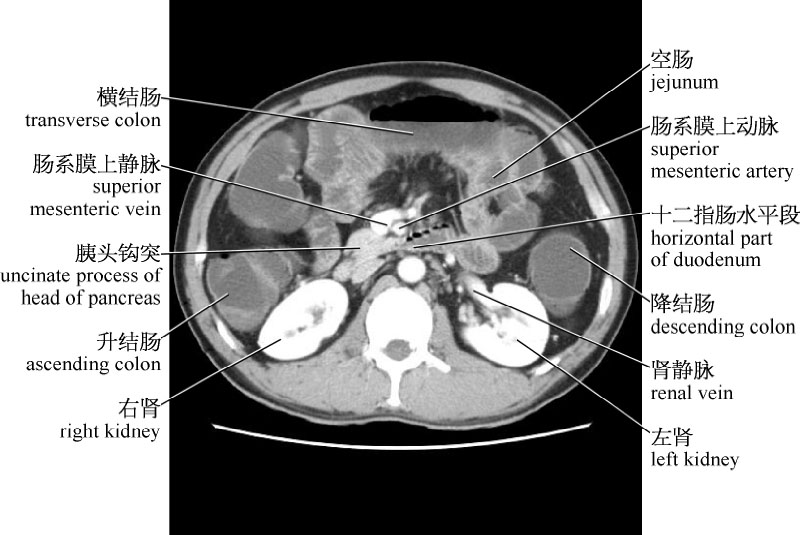
\includegraphics{./images/Image00172.jpg}
 \captionsetup{justification=centering}
 \caption{结肠}
  \end{figure} 
 \FloatBarrier

\begin{figure}[!htbp]
 \centering
 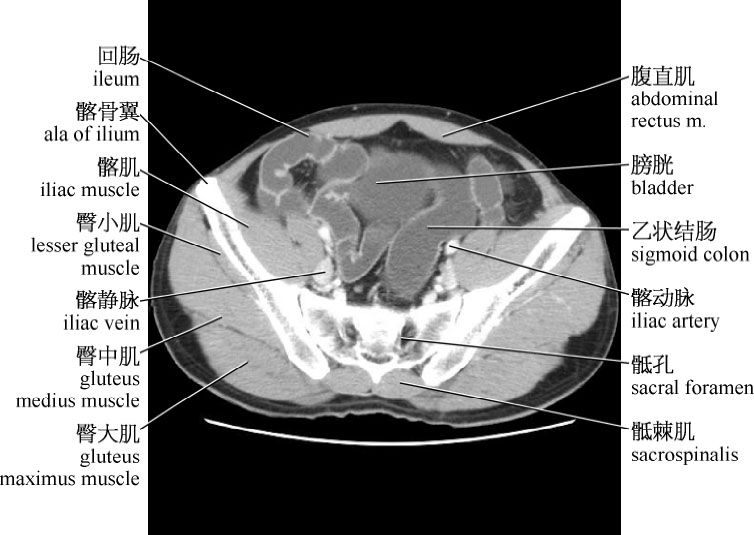
\includegraphics{./images/Image00173.jpg}
 \captionsetup{justification=centering}
 \caption{乙状结肠}
  \end{figure} 
 \FloatBarrier

\begin{figure}[!htbp]
 \centering
 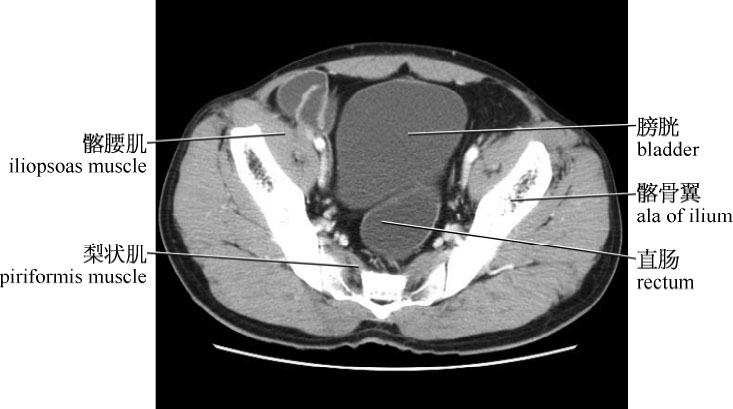
\includegraphics{./images/Image00174.jpg}
 \captionsetup{justification=centering}
 \caption{直肠}
  \end{figure} 
 \FloatBarrier

\section{非轴位影像与仿真内镜}

由于消化道走行迂曲,因此需要使用非轴位(如斜冠状位或斜矢状位等)观察上下走行或斜向走行的消化道结构。

\begin{figure}[!htbp]
 \centering
 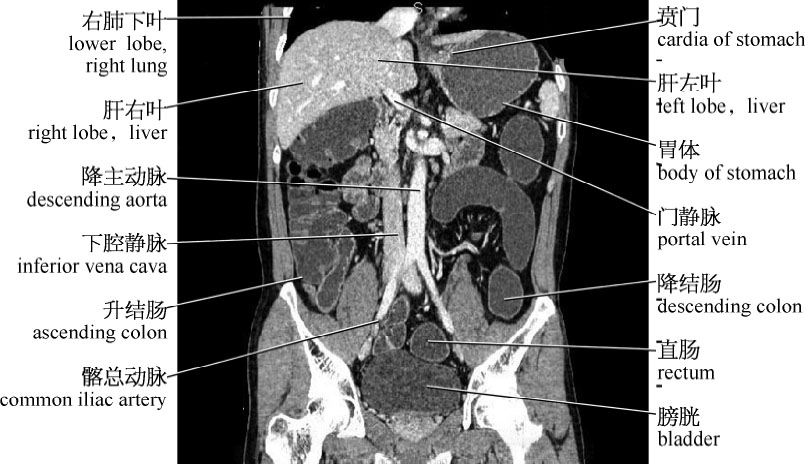
\includegraphics{./images/Image00175.jpg}
 \captionsetup{justification=centering}
 \caption{胃底与贲门}
  \end{figure} 
 \FloatBarrier

\begin{figure}[!htbp]
 \centering
 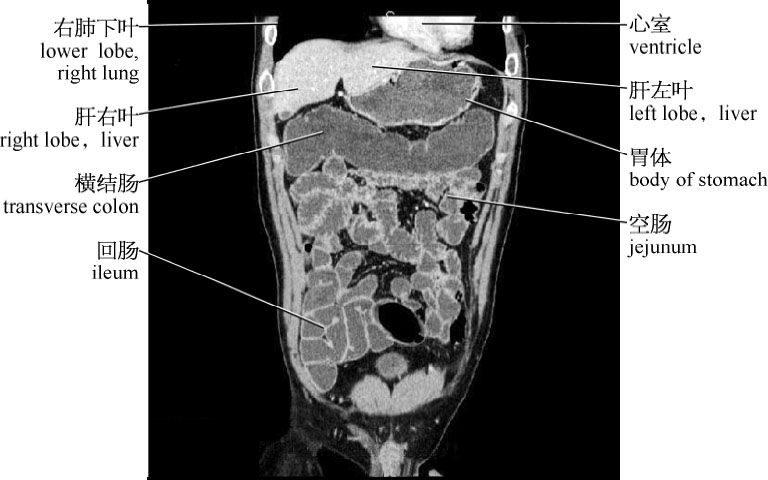
\includegraphics{./images/Image00176.jpg}
 \captionsetup{justification=centering}
 \caption{胃体与横结肠}
  \end{figure} 
 \FloatBarrier

\begin{figure}[!htbp]
 \centering
 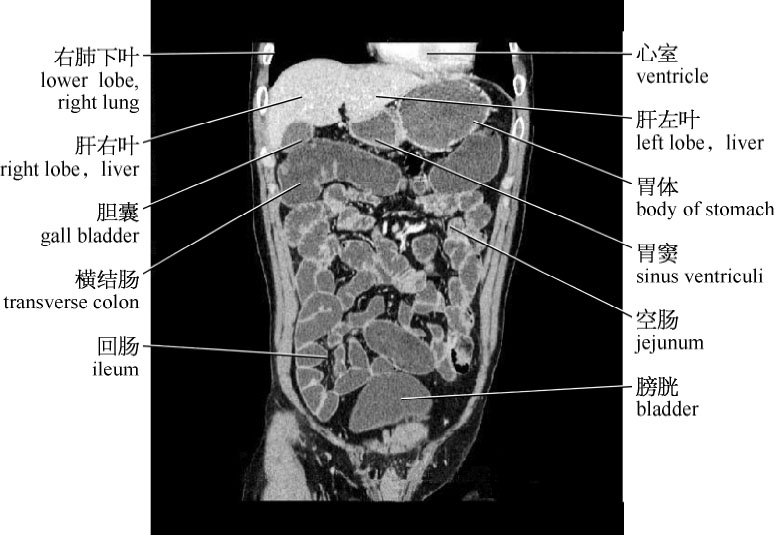
\includegraphics{./images/Image00177.jpg}
 \captionsetup{justification=centering}
 \caption{胃体与胃窦}
  \end{figure} 
 \FloatBarrier

\begin{figure}[!htbp]
 \centering
 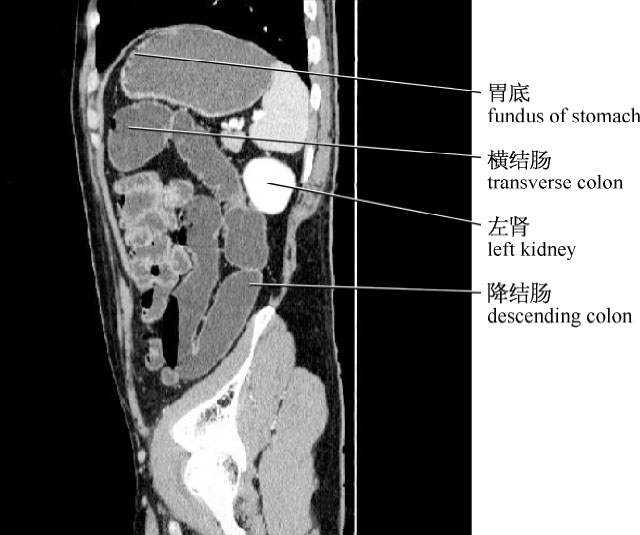
\includegraphics{./images/Image00178.jpg}
 \captionsetup{justification=centering}
 \caption{胃底与左半结肠}
  \end{figure} 
 \FloatBarrier

\begin{figure}[!htbp]
 \centering
 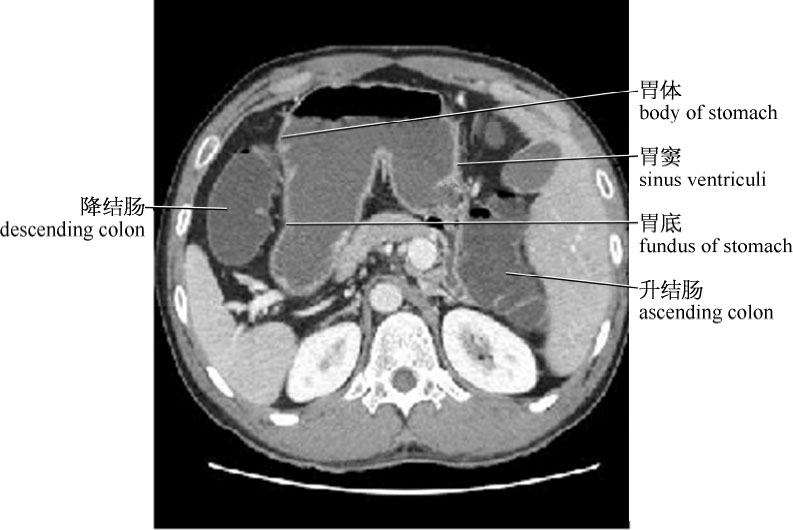
\includegraphics{./images/Image00179.jpg}
 \captionsetup{justification=centering}
 \caption{全胃}
  \end{figure} 
 \FloatBarrier

\begin{figure}[!htbp]
 \centering
 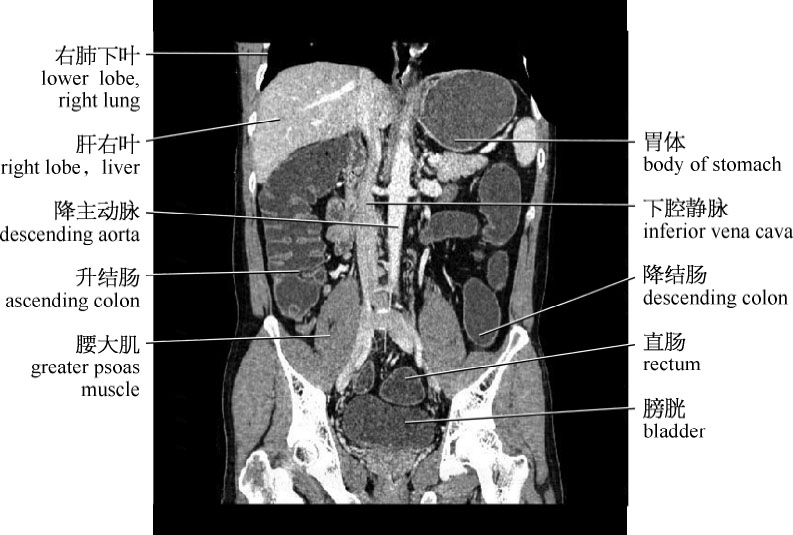
\includegraphics{./images/Image00180.jpg}
 \captionsetup{justification=centering}
 \caption{右半结肠}
  \end{figure} 
 \FloatBarrier

\begin{figure}[!htbp]
 \centering
 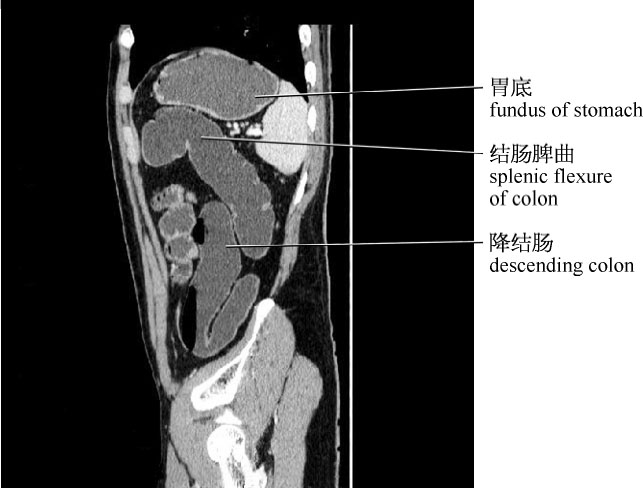
\includegraphics{./images/Image00181.jpg}
 \captionsetup{justification=centering}
 \caption{结肠脾曲}
  \end{figure} 
 \FloatBarrier

\begin{figure}[!htbp]
 \centering
 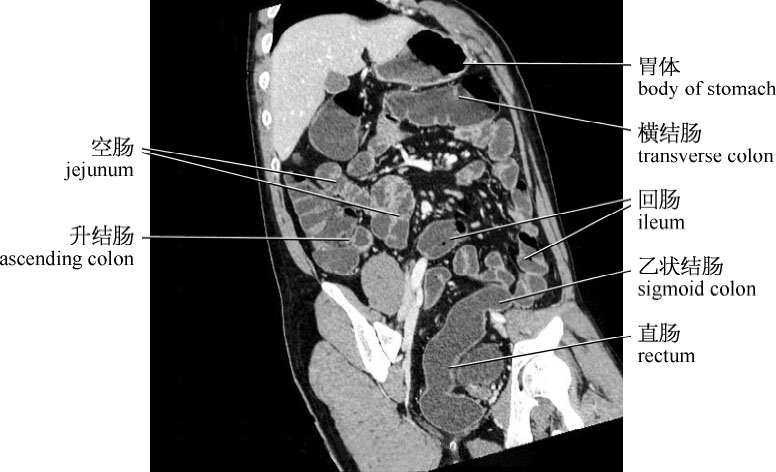
\includegraphics{./images/Image00182.jpg}
 \captionsetup{justification=centering}
 \caption{直肠与乙状结肠}
  \end{figure} 
 \FloatBarrier

\begin{figure}[!htbp]
 \centering
 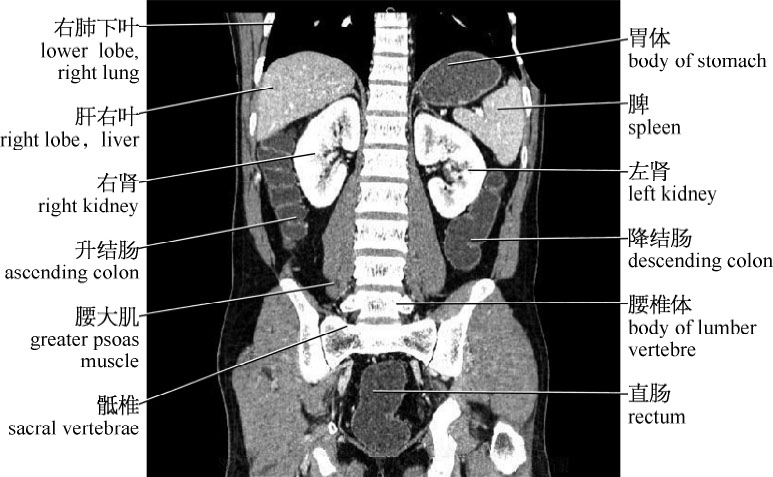
\includegraphics{./images/Image00183.jpg}
 \captionsetup{justification=centering}
 \caption{直肠}
  \end{figure} 
 \FloatBarrier

仿真内镜是目前MSCT较为常用的观察消化道腔内结构的重要重建方法之一,可以直观地显示腔内隆起性病变。

\begin{figure}[!htbp]
 \centering
 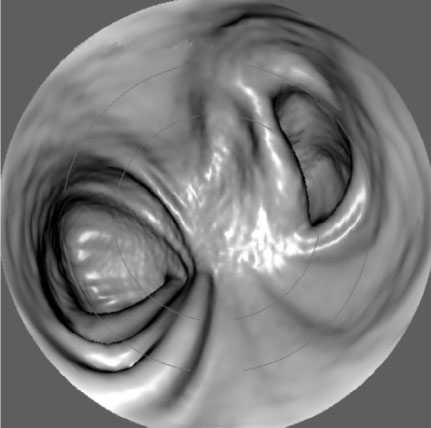
\includegraphics{./images/Image00184.jpg}
 \captionsetup{justification=centering}
 \caption{正常结肠}
  \end{figure} 
 \FloatBarrier

\begin{figure}[!htbp]
 \centering
 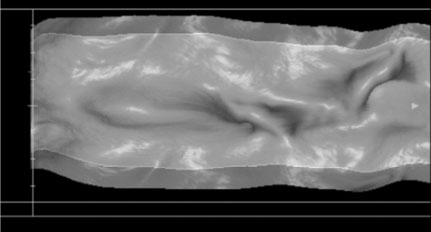
\includegraphics{./images/Image00185.jpg}
 \captionsetup{justification=centering}
 \caption{结肠平铺展示}
  \end{figure} 
 \FloatBarrier

\begin{figure}[!htbp]
 \centering
 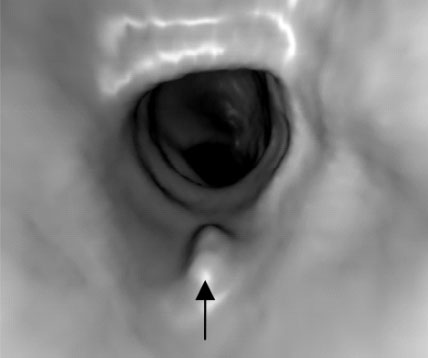
\includegraphics{./images/Image00186.jpg}
 \captionsetup{justification=centering}
 \caption{结肠息肉(箭头)}
  \end{figure} 
 \FloatBarrier